\section{Visual Design} % or "Research Plan"
\label{sec:vis}

Our ultimate goal, is to design a visualization tool for understanding courses interactions. Our target users are professors, students and academic advisors. We talk with graduate students and professors about what they need to summarize our tasks as below:
\begin{itemize}
	\item [T1] Overview of clusters of correlated courses
	\item [T2] For a specific course, find the courses which potentially benefit it and compare the importance of these courses
	\item [T3] For two selected courses, show details of student grades
\end{itemize}

We preprocess our original data and choose to use all the course records of computer science department for our implementations. We carefully select the visualization techniques which can be easily understood by users. Our system has three major view: the adjacency matrix, bar chart view and parallel coordinates view. In this section. We describe all the works we have done and the details of Coursim.%\~\ref{sec:background}

%\You may want to use figures to illustrate your point, such as
%\Figure~\ref{fig:sample}.

\subsection{Data Processing}
\label{sec:data}
Towards this end, we performed a pilot study using student data from a Canadian research university.  This data included all students who had taken a computer science course at that university between September 2001 and December 2011.

The data was in a comma-separated file made up of rows with 6 fields:  a unique, anonymized student identifier, the term (which could be Spring, Summer or Fall and the year), the subject ID (such as “CS” or “ENGL”), the course code (such as “101”), the percentile grade received and the student’s major.

The data needed to be preprocessed in preparation for the similarity calculation and the visualization.  A unique, sequential identifier was added to each line.  There was a variety of identifiers for problems students had in a course, such as “WD” indicating withdrawal, “DNR” indicating the final exam was not written.  These were replaced with 0 so that there would be a consistent, natural number domain for the grades.  Some of the course codes had an optional letter suffix, which would indicate if it was offered on-line or at another campus (for example).  These were removed and all courses with the same code were treated as the same value.

We removed courses and corresponding records which less than 10 students take in the data set on the basis that there was insufficient pairwise to measure the interactions between two courses. After these adjustments, the training set consisted of 37,392 students with data about 468,632 courses they took. There were 2,326 unique courses in the dataset.Specifically, for the computer science department, there are 61 courses, 2861 students, in total 38751 records.


\begin{figure}[h]
	\centering % avoid the use of \begin{center}...\end{center} and use \centering instead (more compact)
	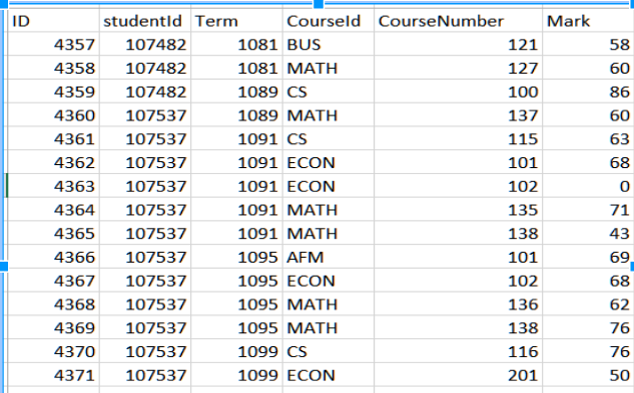
\includegraphics[width=\columnwidth]{figs/data} 
	\caption{Original data table}
	\label{fig:data}
\end{figure}

\subsection{Adjacency Matrix View}
\label{sec:matrix}
The Adjacency Matrix view enables users to grasp a global view of the all the courses. We use D3 library which contains the existing adjacency matrix template~\cite{Bostock:2011:DDD:2068462.2068631}. Each grid in the matrix represents the potential benefits the column course may get from the row course. Each row shows that, for a specific course, all the courses it may have a positive influence on. Each column depicts that, for a chosen course, all the courses which may benefit it. We build a mouse over in this view, when the users move their mouse on the grid, the column and the row associated with that gird chosen will be highlighted with a bold border which will make it easier to obverse the column and the row. The view also consists a zoomable and navigation feature which can be used to filter the uninterested data based on the demand. 

Adjacency Matrix view can clearly show the every possible connection between each pair of courses. Compared to node-link diagram or dagre layout~\cite{Bostock:2011:DDD:2068462.2068631}, it has obvious advantages in terms of recognition and orientation. When the size of the data get big, the force-directed node link diagram or dagre layout will include a lot of cross edges and become messy. It is hard for users to localize the actual pair of courses they want, and identify the actual relations between them. But adjacency matrix can always navigate users to the right pair of data and is easy for users to explore the data set and find interesting patterns. 

The color scale ranging from white to dark red indicates the similarity between each pair of courses. White grids mean either there are less than 10 students or the influence the one course has on the later course is negative. We talk about how we calculate the similarities measurement in the next section.
\begin{figure}[h]
	\centering % avoid the use of \begin{center}...\end{center} and use \centering instead (more compact)
	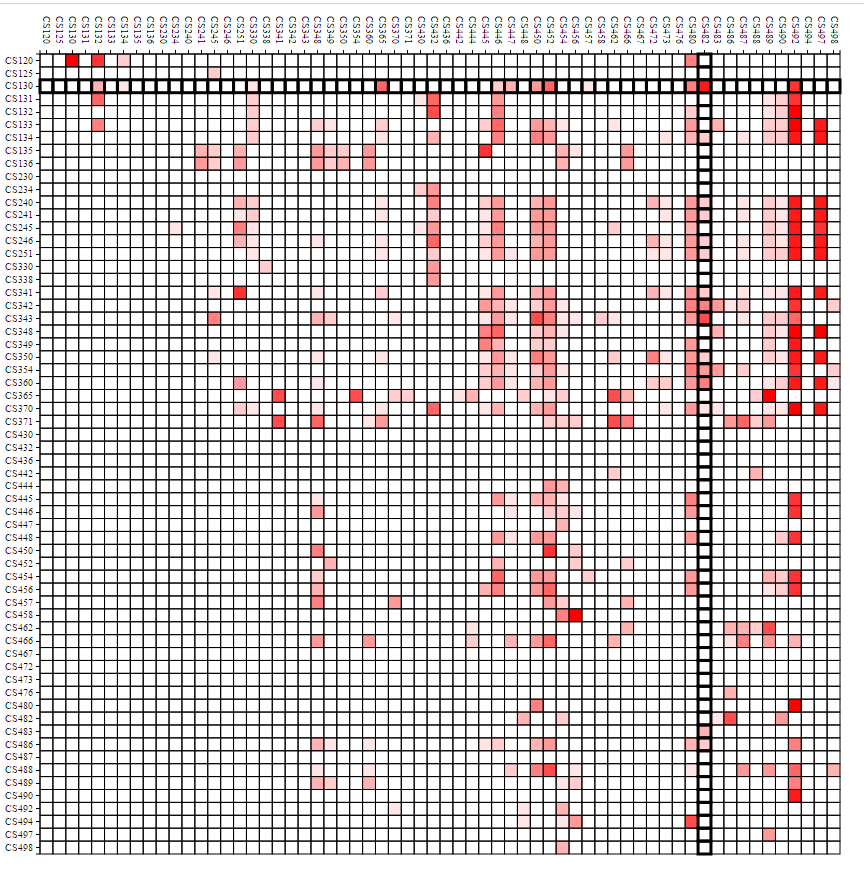
\includegraphics[width=\columnwidth]{figs/matrix} 
	\caption{Adjacency Matrix View}
	\label{fig:sample}
\end{figure}

\subsection{Benefits Measurement}
\label{sec:benefits}
In order to demonstrate the benefits a course(Pre1) may give to another(Course1), we want to build a measurement way based on students’ performance in both of the courses. The intuition is that if a student gets high scores in Pre1 and in the future semesters, they also get a high score in Course1, which may indicate the benefits between Pre1 and Course1. On the contrary, if the high score in Pre1 ends up with bad performance in Course1, the benefits may be few. Pearson-correlation seams a considerable method. But it turns out that it is not suitable in our case. The problem is that if for Pre1 and Course1, we extract the grades of the students who have taken both two courses in sequence and put them into two vectors. The results we get are not convincing. There are a few problems when applying Pearson-correlation. The first is that a lot of students’ performance is consistent. A student who can get high scores in one course will also achieve good scores in later courses. This makes the Pearson-correlation for each course very similar (around 0.7), which is hard to identify the benefits. Another problem is, the distribution of scores for different courses are also different. In some courses, 80 points may have been the one of best performance among all the students. The actual points depend on different professors and the different courses contain diverse standards.

In order to avoid the two problems mentioned above, we introduce a new benefit measurement based on recommender system. The motivation is that if a student(Jack) whose overall performance is not that good gets higher score in Course1 after taking Pre1 than the students whose overall performance are similar to Jack but without taking Pre1, we say Pre1 may be a benefit for course A.  We choose Collaborative Filtering which can predict a student’s grade on one course based on the similarity to other students. More specifically, we choose item-based recommender which is more efficient than the user-based recommenders since we have much fewer courses than the number of students.  To measure the benefit Pre1 may bring to Course1, we do as follows:
\begin{itemize}
	\item Step 1: For each course pair (in order, for example, Pre1, Course1) taken by more than 10 students, remove the actual grades of Course1 of those students and take the rest of the records of the training data. 
	\item Step 2 : Running an Item-based recommender using Pearson Correlation to predict the grades the students will get for Course1.
	\item Step 3: Calculating the average of the differences between the actual and predicted grades and take that as the similarity measurement.
\end{itemize}
\begin{figure}[h]
	\centering % avoid the use of \begin{center}...\end{center} and use \centering instead (more compact)
	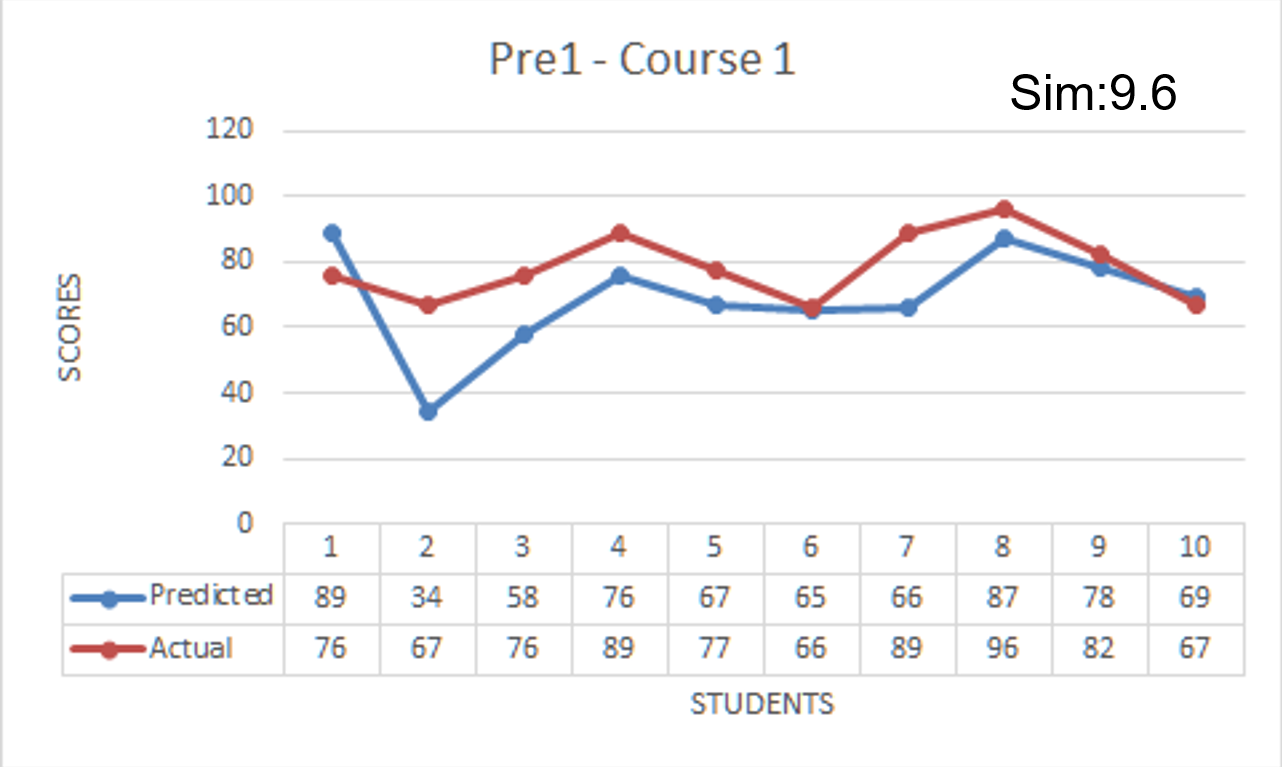
\includegraphics[width=\columnwidth]{figs/measure} 
	\caption{Our method based on item-based recommender system, Pre1 clearly benefit Course1 with a beachmark 9.6}
	\label{fig:sample}
\end{figure}

From Fig. 6, we can clearly see that most of the 10 students who have taken both Pre1 before Course1 have better actual scores than the prediction which is based on the overall performance. In other words, compared with the students whose overall performance is similar but without taking Pre1, these students have gotten 9.6 more points on Course1 averagely, which is a great improvment. Therefore we can say, Pre1 should benefit Course1 even without knowing the contents of both two courses.

This new measurement gives us a better way to measure the actual benefits a course may give to the other. In stead of using Pearsonal Corrleations, it is a more solid way because it can tolerate the influence of the students’ consisitent performance and also avoid the direct comparsion using scores of different courses. Using this method, we get a much better distribution of the overall benefits measurement. Specifically,  for the computer science department, there are 1191 pairs of courses have benefit benchmarks.The benefits points range from -17.9 to 12.6(Fig 7). Minus points mean the negative influence and positive points mean active influence. In the current version of our adjacency matrix , we ignore the negative points, which we also also color it as a difference color. This maybe one of our future work.
\begin{figure}[h]
	\centering % avoid the use of \begin{center}...\end{center} and use \centering instead (more compact)
	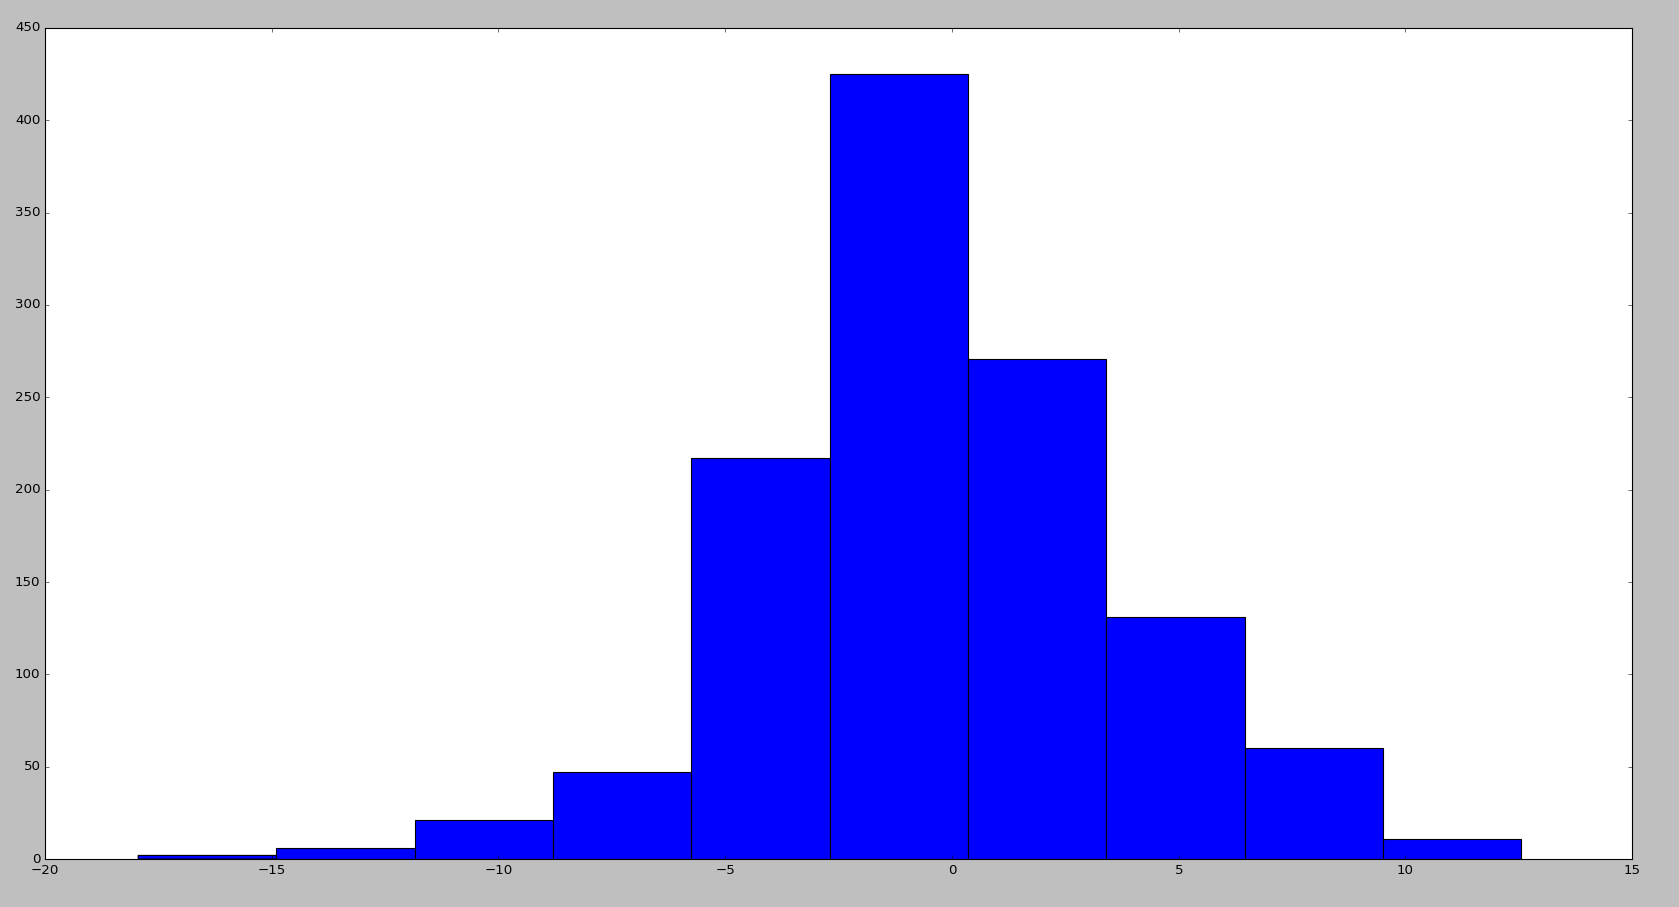
\includegraphics[width=\columnwidth]{figs/markdistribution} 
	\caption{The distribution of benefits benchmarks for CS courses, ranging from -17.9 to 12.6,bigger the number, more benefits may exit}
	\label{fig:sample}
\end{figure}

\subsection{Bar Chart View}
\label{sec:bar}
The bar chart view details the course users are interested in. The interaction is built between the adjacency matrix and the bar chart. When the user finds one course he is interested and wants to see all the courses may benefit this course. They can click on any grid along the column of that course. The bar chart will pop up. It reveal the top 10 courses which may benefits the selected course and order them by the benefit benchmarks. The color of each bar is the same as the corresponding grid in the adjacency matrix to make sure the consistency and.  This style avoid the possible confusion when users are navigating to the bar chart view. Using this bar chart view, users can easily find out for the specific course, which one has the highest benefit benchmark. Also, for a pair of courses, what’s the rank of the pre-course, is that actually a good choice? The view helps users to figure out these problems and make good decision for choosing good prerequisites. 
\begin{figure}[h]
	\centering % avoid the use of \begin{center}...\end{center} and use \centering instead (more compact)
	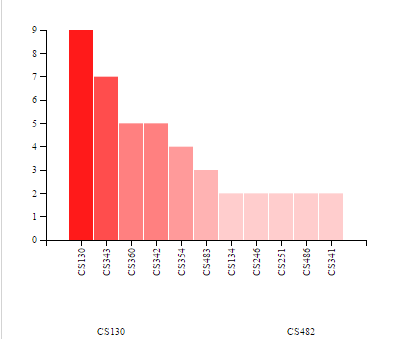
\includegraphics[width=\columnwidth]{figs/barchart} 
	\caption{Bar chart view for course CS482}
	\label{fig:sample}
\end{figure}

\subsection{Parallel Coordinates View}
\label{sec:parallel}
For a pair of courses we are interested in,  we use a parallel coordinates graph to show the specific grades changes for students who have taken both courses. Each line’s start point is the score that a student gets in the previous course, and the end point is the score the same students gets in the later course. The interaction is build between the adjacency matrix and the parallel coordinates. When a gird is clicked, a parallel coordinates will be shown in this view. Instead of focusing on the course level and getting a summarized benchmark  for each pair of courses. The parallel coordinates will allow users to explore the details and show all the trends of each student’s performance between theses two courses. Users can clearly observe the changes of each student which can be  a good reference when they are considering the benefit between two courses. For example ,from Fig. 9, the overall benefit CS240 may bring to CS492 is high positive. But we can also find some obvious outliners: a student getting almost 98 points gets 65 in the CS492, another student whose score for CS240 is 78 ends up getting 8 points in CS492. These are some anomalies which users can easily find out with the parallel coordinates. Fo r the future work, different colors are utilized to show the grade section for the course. And we also need to build  interaction between bar chart and parallel coordinates.
\begin{figure}[h]
	\centering % avoid the use of \begin{center}...\end{center} and use \centering instead (more compact)
	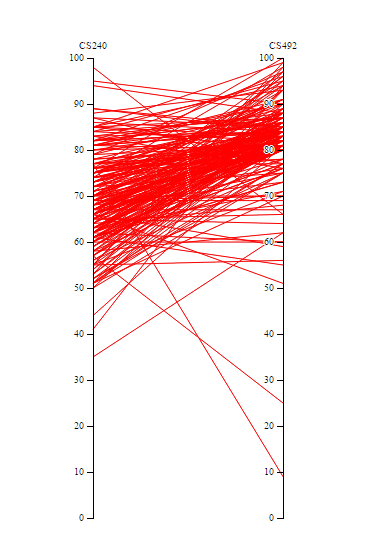
\includegraphics[width=\columnwidth]{figs/parallel} 
	\caption{Parallel coordinates graph for CS240-CS492}
	\label{fig:sample}
\end{figure}

%\begin{figure*}[h]
% \centering 
% 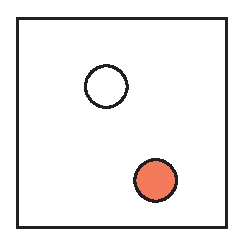
\includegraphics[width=\textwidth]{figs/sample} 
% \caption{Double Column Figure.}
% \label{fig:sample2}
%\end{figure*}

